In this chapter we will walk through three simplified binary PFC models. The
first is the original binary PFC model, which, while highly successful at
modelling a few important phenomena is ultimately limited in scope. The second
is the binary structural phase field crystal, or binary XPFC which was
successful in modelling a broad spectrum of crystalline structures, but was
limited in its ability of model liquid instablilities and a variety of phase
diagrams. Finally, we'll see a new contribution to which we will call the
regular phase field crystal model which is successful in modeling a broad
spectrum of invariant binary reactions and crystalline structures. 

All binary PFC models begin with a multicomponent variant of the approximate
free energy functional established in Chapter \ref{fundamentals},
%
\begin{align}
    \label{binary_cdft_free_energy}
    \beta\F[\A, \B] &= \sum_{i=A, B} \int \mathrm{d}r 
        \,\rho_i(r) \ln\l(\f{\rho_i(r)}{\rho_i^0}\r) 
        - (1 - \beta\mu_i^0)\Delta\rho_i(r)\\
    &- \f{1}{2} \sum_{i,j=A, B} \Delta\rho_i(r) \ast C^{(2)}_{ij}(r, r^\prime) 
        \ast \Delta\rho_j(r^\prime). \nonumber
\end{align}
%
It is convenient to change variables to a dimensionless total density, $n(r)$
and local concentration, $c(r)$,
%
\begin{gather}
    n(r) = \f{\Delta \rho}{\rho_0} = \f{\Delta\A + \Delta\B}{\A^0 + \B^0} \\
    c(r) = \f{\B}{\rho} = \f{\B}{\A + \B}.
\end{gather}
%
Scaling out a factor of the total reference density, $\rho_0$ we can break the
free energy functional in these new variables into three parts,
%
\begin{equation}
    \label{binary_total_free_energy}
    \f{\beta\F[n, c]}{\rho_0} = \f{\beta\F_{id}[n]}{\rho_0} 
        + \f{\beta\F_{mix}[n, c]}{\rho_0}
        + \f{\beta\F_{ex}[n, c]}{\rho_0},
\end{equation}
%
Where,
%
\begin{gather}
    \label{binary_ideal}
    \f{\beta\F_{id}[n]}{\rho_0} =
        \int \mathrm{d}r \,\l\lbrace (n(r) + 1)\ln(n(r) + 1) 
        - (1 - \beta\mu^0)n(r) \r\rbrace \\
    \label{binary_mixing}
    \f{\beta\F_{mix}[n, c]}{\rho_0} =
        \int \mathrm{d}r \,\l\lbrace (n(r) + 1)\l( 
            c\ln\l(\f{c}{c_0}\r) + (1-c)\ln\l(\f{1-c}{1-c_0}\r) \r)\r\rbrace, 
\end{gather}
%
And, if we assume the local concentration $c(r)$ varies over much longer length
scales than the local density $n(r)$,
%
\begin{align}
    \label{binary_excess}
    \f{\beta\F_{ex}[n, c]}{\rho_0}
        = &-\f{1}{2} n(r) \ast \l[ 
            C_{nn}(r, r^\prime) \ast n(r^\prime) 
          + C_{nc}(r, r^\prime) \ast \Delta c(r^\prime)\r] \\
        &-\f{1}{2} \Delta c(r) \ast \l[
            C_{cn}(r, r^\prime) \ast n(r^\prime) 
          + C_{cc}(r, r^\prime) \ast \Delta c(r^\prime)\r]. \nonumber
\end{align}
%
We have introduced $\mu_0$ as the total chemical potential of the reference
mixture, $c_0 = \B^0 / \rho_0$ as the reference concentration and $\Delta c(r)
= c(r) - c_0$ as the deviation of the concentration from the reference.  The
$n-c$ pair correlation introduced in the excess free energy are,
%
\begin{align}
    C_{nn} &= \rho_0\l(c^2 C_{BB} + (1 - c)^2C_{AA} + 2c(1-c)C_{AB}\r) \\
    C_{nc} &= \rho_0\l(c C_{BB} - (1 - c) C_{AA} + (1 - 2c)C_{AB}\r) \\
    C_{cn} &= C_{nc} \\
    C_{cc} &= \rho_0\l(C_{BB} + C_{AA} - 2 C_{AB}\r)
\end{align}
%
Explicit calculations can be found in Appendix \ref{binary_correlations}.
Differences in the various simplified binary PFC theories stem from differing
approximations of the terms in the free energy stated in equation
\ref{binary_total_free_energy}.

%%%%%%%%%%%%%%%%%%%%%%%%%%%%%%%%%%%%%%%%%%%%%%%%%%%%%
\section{Original Binary Phase Field Crystal Model} %
%%%%%%%%%%%%%%%%%%%%%%%%%%%%%%%%%%%%%%%%%%%%%%%%%%%%%

In the original simplified binary PFC theory, all terms in the free energy are
expanded about $n(r) = 0$ and $c(r) = c_0$ (ie., about their reference states).
For the ideal free energy this results in a polynomial truncated to fourth
order,
%
\begin{equation}
    \f{\beta\F_{id}[n]}{\rho_0} = \integrate{r}
    \l\lbrace \f{n(r)^2}{2} - \f{n(r)^3}{6} + \f{n(r)^4}{12} \r\rbrace.
\end{equation}
%
The linear term is dropped due to invariance in the equations of motion. If we
assume for simplicity of demonstration $c0 = 1/2$, the free energy of mixing
becomes a simple fourth order polynomial as well,
%
\begin{equation}
    \f{\beta\F_{mix}[n, c]}{\rho_0} = \integrate{r} \l\lbrace
       2\Delta c(r)^2 + \f{4\Delta c(r)^4}{3}
    \r\rbrace.
\end{equation}
%
Linear couplings to $n(r)$ are dropped by assuming, as we already have, that
the concentration field varies on a much longer length scale than the total
density and noting that the total density is defined about its average. This
argument can also be applied the linear couplings to $n(r)$ in the excess free
energy term which leaves only the $C_{nn}$ and $C_{cc}$ terms. Finally, these
two terms are approximated with a gradient expansions of the correlation
functions,
%
\begin{gather}
    C_{nn}(r, r^\prime) = \d(r - r^\prime)\l(
        \alpha + \beta \nabla^2 + \gamma \nabla^4 + \dots\r), \\
    C_{cc}(r, r^\prime) = \d(r - r^\prime)\l(
        \epsilon + \xi \nabla^2 + \dots\r).
\end{gather}
%
The expansion parameters, $\alpha, \beta,$ and $\gamma$ are all dependent on
temperature and concentration. We are required to expand $C_{nn}$ to fourth
order because, as noted in chapter \ref{dft_of_freezing} the peak of the direct
correlation function in Fourier space is the driving force for solidification.
The concentration field is correlated over a longer length scale implying that
only the short wavevectors are important in $C_{cc}$ so we can expand just to
quadratic order.

Gathering terms the resulting free energy functional for the original simplified
binary PFC model\footnote{The orignal simplified binary PFC model was
expressed using slightly different variables. We expand in $\Delta c(r)$ here to 
facilitate comparison with other theories} is,
%
\begin{align}
    \f{\beta\F[n, c]}{\rho_0} &= \integrate{r} \l\lbrace 
        \f{1}{2} n(r) \l( 1 - \alpha - \beta\nabla^2 - \eta\nabla^4 \r) n(r)
      - \f{n(r)^3}{6} + \f{n(r)^4}{12} \r\rbrace \\
    &+ \integrate{r} \l\lbrace
        \f{1}{2} \Delta c(r) \l( 4 - \epsilon - \xi\nabla^2 \r) \Delta c(r) 
      + \f{4 \Delta c(r)^4}{3} \r\rbrace. \nonumber
\end{align}
%

The strength of the original simplified binary PFC model is that is retains
most of the important physics of binary alloys in a very reduced theory. For
instance, the simplified model is capable of describing the equilibrium phase
diagrams of both eutectic alloys alloys and materials with a solid state
spinodal / liquid minimum.  Supplied with a diffusive equation of motion the
simplified model can model an impressive diversity of dynamic phenomena
including eutectic growth, phase segregation, dendritic growth, dislocation
motion in solid state spinodal coarsening and epitaxial growth.

The major limitation of the original simplified model is that the gradient
expansion of the 

{   
    \color{ForestGreen} List all of the applications which the original model,
    in its various forms, was successfully applied to. List failures if
    possible (here I'm specifically thinking about the Karma fitting problem
    for iron) and conceptual problems about modelling differect structures. 

    Additionally note the limitations of expansions in the 'concentration' when
    attempting to reproduce realistic phase diagram. Essentially, the divergent
    behaviour at the concentration boundaries makes this behaviour work.
}



%%%%%%%%%%%%%%%%%%%%%%%%%%%%%%%%%%%%%%%%%%%%%%%%%%%%%%%
\section{Binary Structural Phase Field Crystal Model} %
%%%%%%%%%%%%%%%%%%%%%%%%%%%%%%%%%%%%%%%%%%%%%%%%%%%%%%%

{
    \color{ForestGreen} Derive the Binary XPFC free energy and note differences
    from the derivation used for the original simplified model. List all of the
    novel applications that where approached using this model. List the theoretical
    advantages (better phase diagrams, precise control of structure etc)

    List disadvantages (liquid is ideal, narrow spectrum of phase diagrams can
    be reproduces). List theoretic disadvantages (ideal mixing instead of more
    realistic regular mixing basically).
}

%%%%%%%%%%%%%%%%%%%%%%%%%%%%%%%%%%%%%%%%%%%%%
\section{Regular Phase Field Crystal Model} %
%%%%%%%%%%%%%%%%%%%%%%%%%%%%%%%%%%%%%%%%%%%%%

{
    \color{ForestGreen} Derive the regular model and show how it is a combination of
    the XPFC and original model. Discuss the way in which this has the advantages
    of each in one theory. Lead into discussion of various equilibrium properties
    of example systems.

}

%%%%%%%%%%%%%%%%%%%%%%%%%%%%%%%%%%%%%
\subsection{Equilibrium Properties} %
%%%%%%%%%%%%%%%%%%%%%%%%%%%%%%%%%%%%%

Here we'll explore the flexibility of the simplified regular PFC model in 
describing various material phase diagrams in binary systems.

%%%%%%%%%%%%%%%%%%%%%%%%%%%%%%%%%%%%%%%%
\subsubsection{Eutectic Phase Diagram} %
%%%%%%%%%%%%%%%%%%%%%%%%%%%%%%%%%%%%%%%%

While previous PFC models have shown that elastic energy is a sufficient
driving force for eutectic solidification our simplified regular model allows
for the examination of the role enthalpy of mixing can play in eutectic solids.
For instance, Murdoch and Schuh noted that in nanocrystalline binary alloys,
while a positive enthaply of segregation can stabilize against grain growth via
solute segregation at the grain boundary, if the enthaply of mixing becomes too
large this effect can be negated by second phase formation or even macroscopic
phase seperation\cite{MURDOCH13}. 

To specialize our simplified regular model to the case of the binary eutectic
we must choose an appropriate model for the correlation function. Choosing an
$\alpha$ phase around $c = 0$ and $\beta$ phase around $c = 1$, we can recover
the pair correlation function used in the original binary XPFC with a
particular choice of window functions: 
%
\begin{align}
   \chi_\alpha(c) &= 2c^3 - 3c^2 + 1 \\
   \chi_\beta(c) &= \chi_\alpha(1 - c).
\end{align}
%
Should we choose, for example, an $\alpha$ and $\beta$ phase with 2 dimensional
hexagonal lattices, differing only by lattice constants, we can produce a phase
diagram like that in Fig. \ref{eutectic}.  

\begin{figure}[h]
    \centering	
    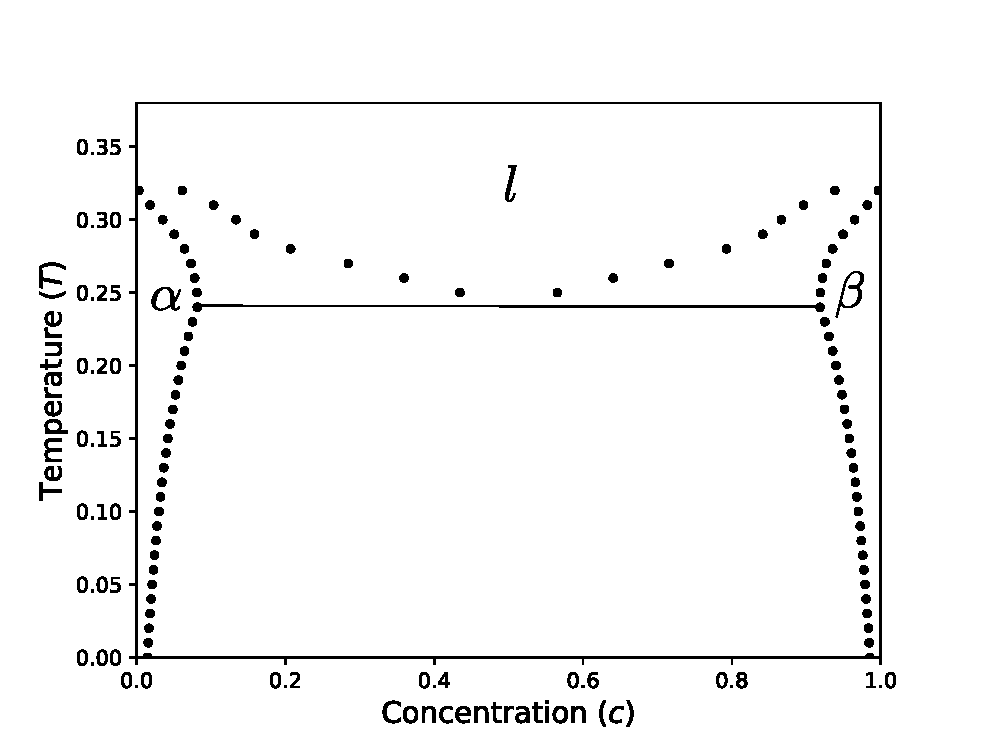
\includegraphics[scale=0.7]{eutectic}
    \caption{
        \label{eutectic} Eutectic phase diagram triangle $\alpha$ and $\beta$
        phases. The free energy parameter are $\eta = 2$, $\chi = 1$,
        $\omega=0.30$, $\epsilon_0 = 3$ and $T_c = 0.01$. The parameters of the
        structure functions are $\alpha_{10\alpha} = \alpha_{10\beta} = 0.8$,
        $k_{10\alpha} = 2\pi$, $k_{10\beta} = 4\pi/\sqrt{3}$ and $T_0 = 1$
    }
\end{figure}

%%%%%%%%%%%%%%%%%%%%%%%%%%%%%%%%%%%%%%%%%
\subsubsection{Syntectic Phase Diagram} %
%%%%%%%%%%%%%%%%%%%%%%%%%%%%%%%%%%%%%%%%%

Our regular model also allows for the study of a variety of invariant binary
reactions that, to date, have not been studied using phase field crystal
models. One such reaction is the syntectic reaction. 

The syntectic reaction, $l_1 + l_2 \rightarrow \alpha $, consists of
solidification at the interface of two liquids. We can achieve this with our
model by setting the spinodal temperature, $T_c$, sufficiently high and
producing a density-density correlation function that is peaked at a
concentration below the spinodal. This can be done by choosing a window
function that is centered about an intermediate concentration, $c_\alpha$ of
the solid phase, $\alpha$. 
%
\begin{equation}
  \chi(c) = e^{- \f{(c - c_\alpha)^2}{2 \alpha_c}}
\end{equation}
%
The resulting correlation function for a hexagonal lattice in two dimensions,
for example, would be,
%
\begin{equation}
  \tilde{C}_{nn}(k; c) = 
    e^{-\f{(c - c_\alpha)^2}{2 \alpha_c}}
    e^{-\f{T}{T_0}} 
    e^{-\f{(k - k^\prime)^2}{2\alpha^2}}
\end{equation}
%
A phase diagram that produces a syntectic reaction with an appropriate choice
of parameters can be seen in Fig. \ref{syntectic}.

\begin{figure}
    \centering
	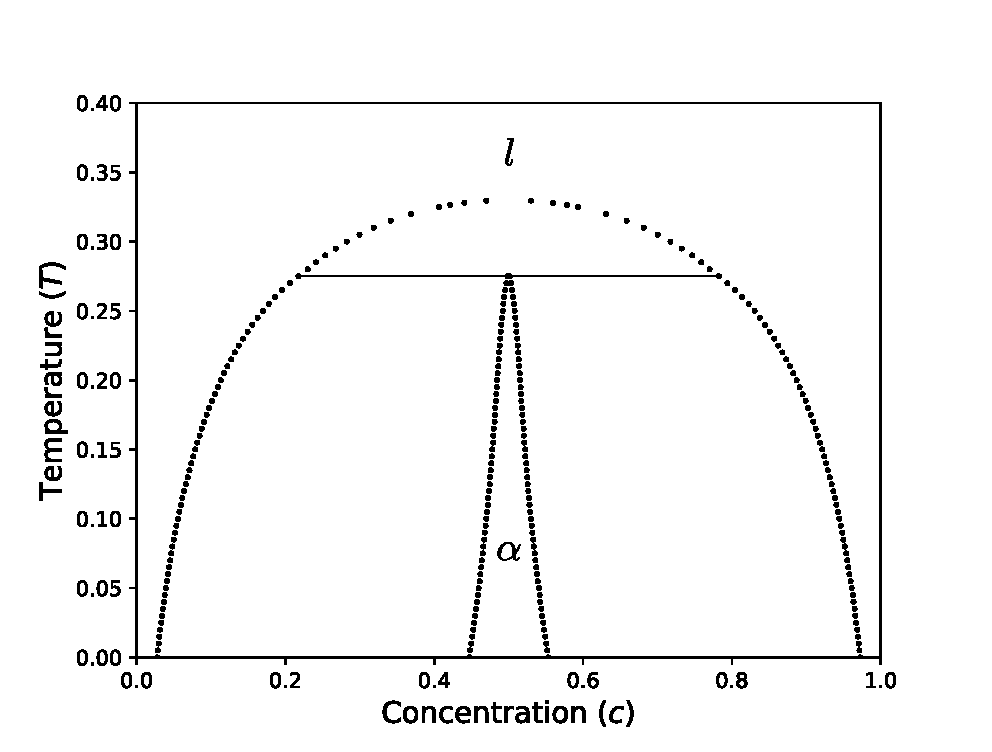
\includegraphics[scale=0.7]{syntectic.eps}
	\caption{
        \label{syntectic} Phase Diagram of Syntectic Alloy with a hexagonal
        $\alpha$ phase. The free energy parameters are $\eta=2$, $\chi=1$,
        $\omega=0.3$, $\epsilon_0 = 10$ and $T_c=0.35$. The parameters for the
        structure function are $\alpha_{10\alpha} = 0.8$, $k_{10\alpha} = 2\pi$
        and $T_0 = 1$
    }
\end{figure}

%%%%%%%%%%%%%%%%%%%%%%%%%%%%%%%%%%%%%%%%%%
\subsubsection{Monotectic Phase Diagram} %
%%%%%%%%%%%%%%%%%%%%%%%%%%%%%%%%%%%%%%%%%%

The monotectic reaction is another invariant binary reaction that has not
previously been studied using PFC models. The monotectic reaction, $l_1
\rightarrow \alpha + l_2$, consists of decomposing liquid into a solute poor
solid and solute rich liquid. To model a monotectic using our regular model we
hypothesize a solid phase at $c=0$ and set the spinondal temperature higher
than the solidification temperature. To achieve this we use a window function
peaked around $c = 0$,
%
\begin{equation}
    \chi_\alpha(c) = e^{-\f{c^2}{2\alpha_c^2}}.
\end{equation}
%
Again considering a simple hexagonal lattice for the $\alpha$ phase, we can
produce a phase diagram with a monotectic reaction with an appropriate choice
of parameters as in Fig. \ref{monotectic}.

\begin{figure}
    \centering
	\includegraphics[scale=0.7]{monotectic.eps}
	\caption{
        \label{monotectic} Phase Diagram of Monotectic Alloy with hexagonal
        $\alpha$ phase. The free energy parameters are $\eta = 2$, $\chi=1$,
        $\omega=0.3$, $\epsilon_0 = 10$, $T_c = 0.35$ and $c_0 = 0.75$. The
        parameters for the structure function are $\alpha_{10\alpha} = 0.8$,
        $k_{10\alpha} = 2\pi$ and $T_0 = 1$ and the parameter for the window
        function is $\alpha_c = 0.4$
    }
\end{figure}

%%%%%%%%%%%%%%%%%%%%%%%%%%%%%%%%%%%%%%%%%%%%%
\subsubsection{Precipitation from Solution} %
%%%%%%%%%%%%%%%%%%%%%%%%%%%%%%%%%%%%%%%%%%%%%

We can also model precipitation of nanoparticles from solution. While on its
surface the equilibrium phase diagram of a solution is that of a simple
solid-liquid coexistance, in practice the metastable features of the phase
diagram can have profound implications on the nucleation kinetics of
precipitate. As an example, precipitation from solution is a typical synthesis
technique for gold and silver nanoparticles. Recent work by Loh \textit{et al}
shows that a metastable spinodal may be playing an important role in the growth
and nucleation of gold nanoparticles under certain diffusive circumstances.

Using the regular XPFC model we can reproduce the condition of a metastable
liquid spinodal underneath the liquid-solid coexistance curve. The approach to
produce a phase diagram is the same as that of of a monotectic, with the
exception that the spinodal temperature, $T_c$, most now be sufficiently low to
be buried underneath the coexistance curve. In keeping with the concentration
being that of the solute, we'll also center the gaussian window function about
$c = 1$. An example, including metastable spinodal, can be seen in Fig.
\ref{precip}.

\begin{figure}
    \centering	
    \includegraphics[scale=0.6]{solution.eps}
	\caption{
        \label{precip} Phase Diagram of Solution \color{ForestGreen} fill
        me in please!!
    }
\end{figure}


{
    \color{ForestGreen} Conclude the chapter with discussion of where what we've
    seen and lead into the discussion for the next chapter of dynamics and
    applications of this theory to more than just simple equilibrium 
    phase diagrams
}
